% Schematic representation of mach zender interferometer
% Modified from a version created by Henrik Kröger, https://github.com/derhedwig/fiberoptics/blob/master/auswertung.tex
% Author: Orlando Torres (2016)

\documentclass{standalone}
\usepackage{amsmath} % Required for \varPsi below
\usepackage{tikz,pgfplots}
\usetikzlibrary{calc}
\usetikzlibrary{patterns}

\begin{document}
  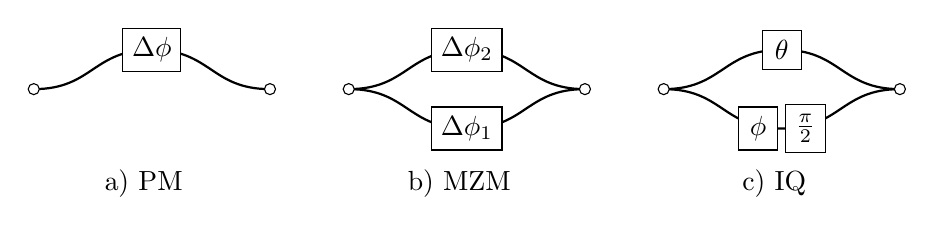
\begin{tikzpicture}
      \definecolor{bbblue}{rgb}{0.964, 0.866, 0.474}
    \definecolor{rrred}{rgb}{0.952, 0.815, 0.105}
    \definecolor{yyyellow}{rgb}{0.925, 0.807, 0.454}    
    %0.933, 0.756, 0.227
    \definecolor{lblue}{rgb}{0.352, 0.556, 0.886}
    \definecolor{sblue}{rgb}{0.607, 0.733, 0.929}
	\definecolor{lyel}{rgb}{0.925, 0.827, 0.152}
    %\definecolor{bbblue}{rgb}{0.070, 0.568, 0.298}
    %\definecolor{rrred}{rgb}{0.933, 0.227, 0.286}
    %\definecolor{yyyellow}{rgb}{0.925, 0.807, 0.454}    
    %0.933, 0.756, 0.227
    %\definecolor{lblue}{rgb}{0.352, 0.556, 0.886}
    %\definecolor{sblue}{rgb}{0.607, 0.733, 0.929}
	%\definecolor{lyel}{rgb}{0.925, 0.827, 0.152}
    
    %define coordinates for modulator (upper side)
    
    %%%%%%%PHASE MODULATOR
    \coordinate (inPM) at (-50mm, 0);
    \coordinate (PBPM) at (-35mm, 5mm);
	\coordinate (PBlPM) at (-35mm, -5mm);
    \coordinate (outPM) at (-20mm, 0mm);
    
    %%%%%% MZ MODULATOR
    \coordinate (inMZM) at (-10.0mm, 0);
    \coordinate (PBpMZM) at (+5mm, -5mm);
    \coordinate (PBnMZM) at (+5mm, 5mm);
    \coordinate (outMZM) at (+20mm, 0mm);    
    
    %%%%%% IQMODULATOR
	\coordinate (inIQ) at (+30.0mm, 0);
    \coordinate (PBpIQ) at (+45mm, -5mm);
    \coordinate (PBnIQ) at (+45mm, 5mm);
	\coordinate (pihalfIQ) at (+50mm, -5mm);
    \coordinate (outIQ) at (+60mm, 0mm); 
    
    %Location of the Signal/Ground/Signal indicators
    \coordinate (phmod) at (-20mm, 4mm);
    \coordinate (gen) at (0mm, 0);
    %\coordinate (gen1) at ($ (gen) + (0, 15mm) $);
    %\coordinate (gen2) at ($ (gen) + (0, -15mm) $);
    \coordinate (ter) at (12mm, 0);
     %Location of the arrow polarization indicators
    \coordinate (arr0) at (-10mm,-13mm);
    \coordinate (arr1) at (-10mm,13mm);
    \coordinate (arrRF0p) at (7.5mm,-15mm);
    \coordinate (arrRF1p) at (7.5mm,-4mm);
    \coordinate (arrRF0+n) at (7.5mm,15mm);
    \coordinate (arrRF1n) at (7.5mm,4mm);
    
    

	%optical paths    
	%Phse Modulator
    \draw[thick,color=black] (inPM) .. controls ($(inPM)  + (7.5mm, 0mm)$) and ($(PBPM)  + (-7.5mm, 0mm)$) .. (PBPM)
    						.. controls ($(PBPM)  + (7.5mm, 0mm)$) and ($(outPM)  + (-7.5mm, 0mm)$) .. (outPM);

	%\draw[thick,color=black] (inPM) .. controls ($(inPM)  + (7.5mm, 0mm)$) and ($(PBlPM)  + (-7.5mm, 0mm)$) .. (PBlPM) 
	%					.. controls ($(PBlPM)  + (7.5mm, 0mm)$) and ($(outPM)  + (-7.5mm, 0mm)$) .. (outPM);
	%MZM Modulator
	\draw[thick,color=black] (inMZM) .. controls ($(inMZM)  + (7.5mm, 0mm)$) and ($(PBpMZM)  + (-7.5mm, 0mm)$) .. (PBpMZM) 
						.. controls ($(PBpMZM)  + (7.5mm, 0mm)$) and ($(outMZM)  + (-7.5mm, 0mm)$) .. (outMZM);
	\draw[thick,color=black] (inMZM) .. controls ($(inMZM)  + (7.5mm, 0mm)$) and ($(PBnMZM)  + (-7.5mm, 0mm)$) .. (PBnMZM) 
						.. controls ($(PBnMZM)  + (7.5mm, 0mm)$) and ($(outMZM)  + (-7.5mm, 0mm)$) .. (outMZM);

	%IQ Modulator
	\draw[thick,color=black] (inIQ) .. controls ($(inIQ)  + (7.5mm, 0mm)$) and ($(PBpIQ)  + (-7.5mm, 0mm)$) .. (PBpIQ) 
						.. controls ($(PBpIQ)  + (7.5mm, 0mm)$) and ($(outIQ)  + (-7.5mm, 0mm)$) .. (outIQ);
	\draw[thick,color=black] (inIQ) .. controls ($(inIQ)  + (7.5mm, 0mm)$) and ($(PBnIQ)  + (-7.5mm, 0mm)$) .. (PBnIQ) 
						.. controls ($(PBnIQ)  + (7.5mm, 0mm)$) and ($(outIQ)  + (-7.5mm, 0mm)$) .. (outIQ);
    

    %inputs/outputs
    \filldraw [black,fill=white] (inPM) circle (2pt);
    \filldraw [black,fill=white] (outPM) circle (2pt);

    \filldraw [black,fill=white] (inMZM) circle (2pt);
    \filldraw [black,fill=white] (outMZM) circle (2pt);

    \filldraw [black,fill=white] (inIQ) circle (2pt);
    \filldraw [black,fill=white] (outIQ) circle (2pt);
      %\draw  [baseline=-0.5ex]\draw[fill=orange,radius=1.5pt] (0,0) circle ;
%\node [shape=circle, minimum width=0mm, minimum height=1mm, color=black, fill=white, draw]
%   	    (inPMi) at (inPM) {};
    
    % Substrate, modulators, Waveguides, MMI and converters %
    
  \node [shape=rectangle, minimum width=3mm, minimum height=3mm, color=black, fill=white, draw]
   	    (phasePM) at (PBPM) {$\Delta\phi$};
 \node [shape=rectangle, minimum width=5mm, minimum height=5mm, color=black, fill=white, draw]
   	    (phasepMZM) at (PBpMZM){$\Delta\phi_1$};
 \node [shape=rectangle, minimum width=5mm, minimum height=5mm, color=black, fill=white, draw]
   	    (phasenMZM) at (PBnMZM) {$\Delta\phi_2$};
 \node [shape=rectangle, minimum width=5mm, minimum height=5mm, color=black, fill=white, draw]
   	    (phaseiQ) at ($(PBpIQ)  + (-3mm, +0mm)$)  {$\phi$};
 \node [shape=rectangle, minimum width=5mm, minimum height=5mm, color=black, fill=white, draw]
   	    (phaseqIQ) at (PBnIQ) {$\theta$};
 \node [shape=rectangle, minimum width=5mm, minimum height=5mm, color=black,, fill=white, draw]
   	    (pihalfIQ) at ($(pihalfIQ)  + (-2mm, 0mm)$) {$\frac{\pi}{2}$};

    \draw (PBPM) node (Phase) [text width=10mm] at +(-1mm, -17mm) {a) PM};
    \draw (PBpMZM) node (MZ) [text width=15mm] at +(0mm, -7mm) {b) MZM};
	\draw (PBpIQ) node (IQ) [text width=10mm] at +(0mm, -7mm) {c) IQ};

  \end{tikzpicture}
\end{document}